\documentclass{article}
\usepackage{graphicx}


\title{The title}

\author{the Author}

\date{\today}

\begin{document}

\maketitle


\begin{abstract}
\label{sec:abstract}
    the abstract goes here
\end{abstract}

\section{Introduction}
\label{sec:intro}


\subsection{sth else}

\subsection*{another sub section}
but without numbering

I can use \\label and \\ref to automatically label and reference things
respectively. As specified in \ref{sec:intro}.

Needs two runs of the compiler for references  to work.

\textbackslash eqref is provided by amsmath

graphics require the graphicx package, included with the \textbackslash includegraphics command

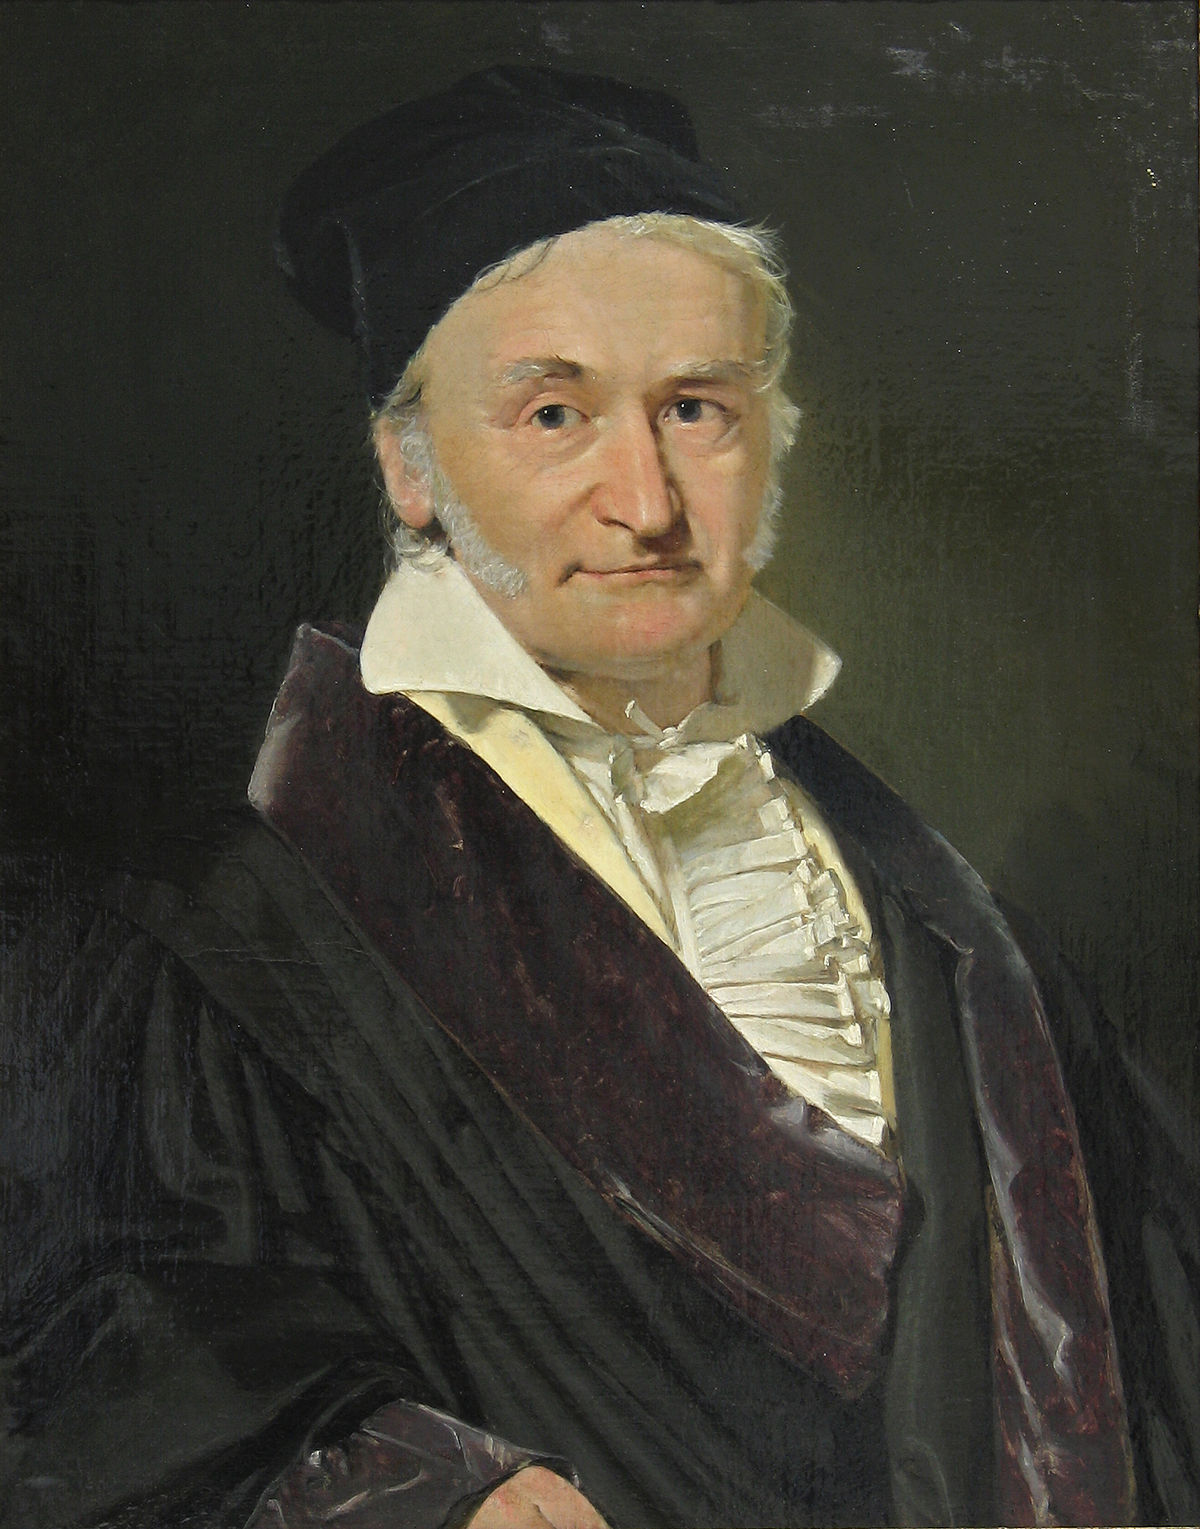
\includegraphics[width=0.5\textwidth]{gauss.jpeg}

square brackets \[ \] are for optional arguments.

\textbackslash document also accepts optional arguments

You can allow latex to decide where the figure can go (it can float)

\begin{figure}
\centering
    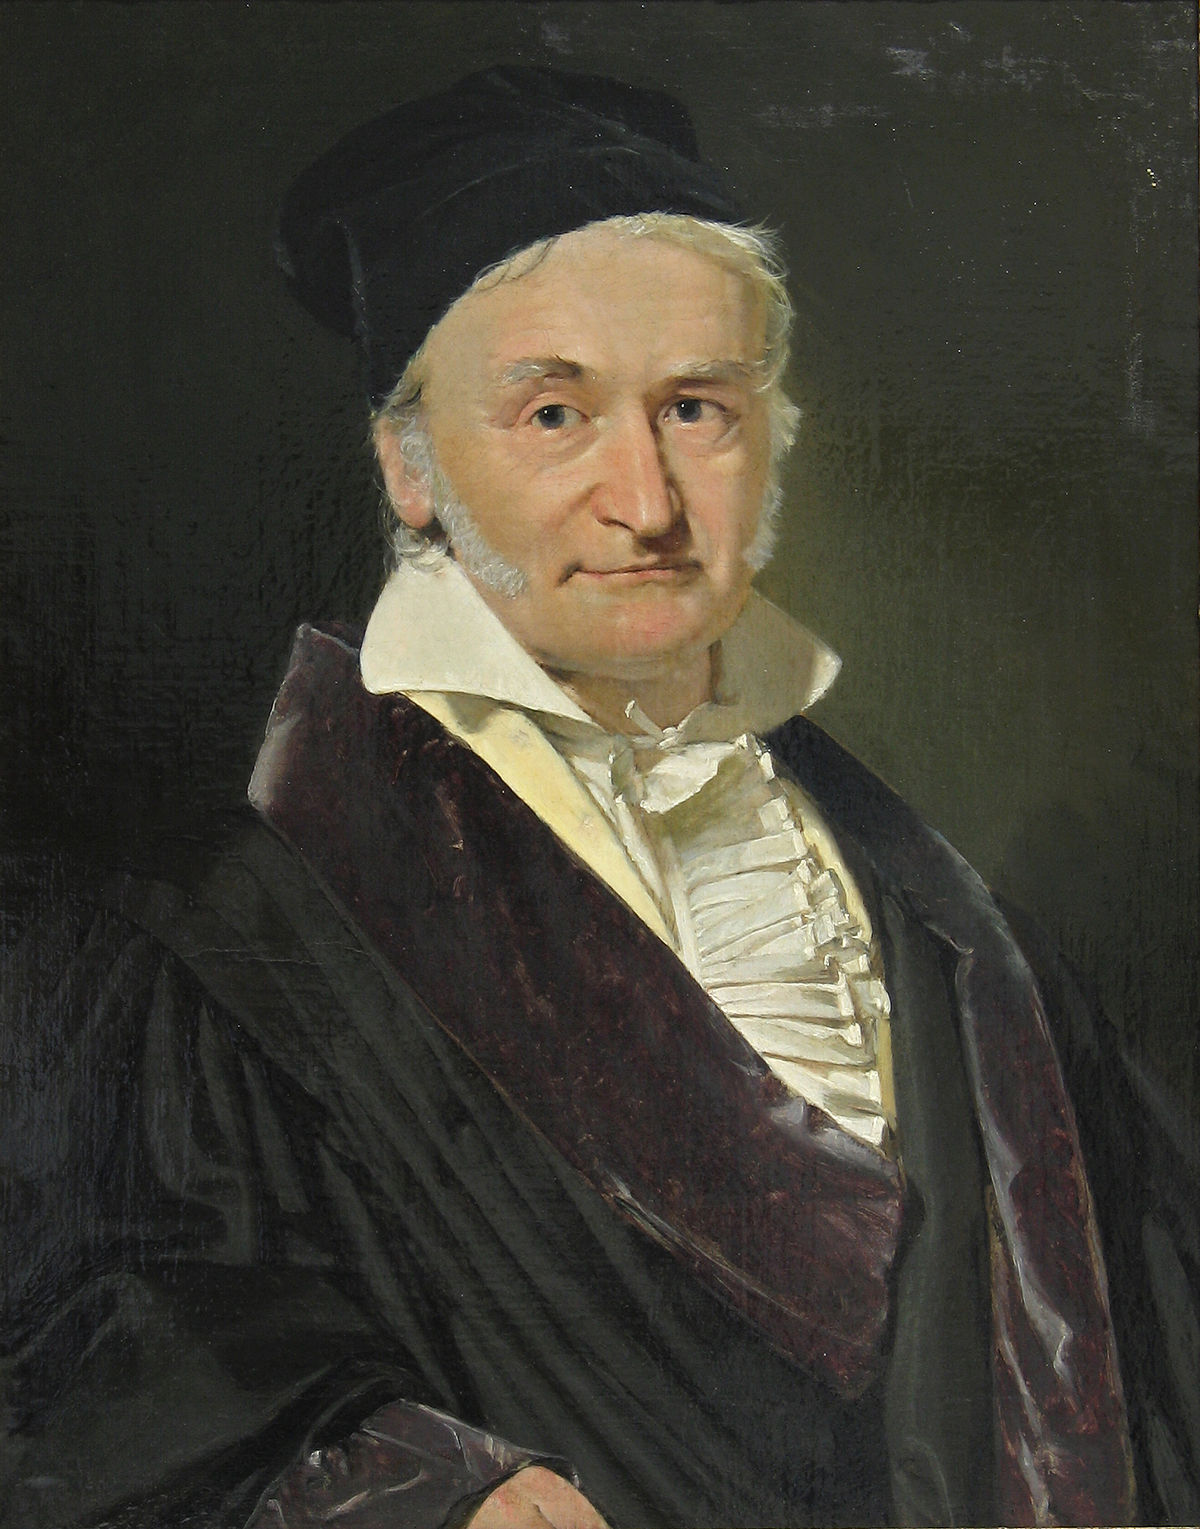
\includegraphics[width=.5\textwidth]{gauss.jpeg}
\caption{\label{fig:gauss}. Que tipazo}
\end{figure}

Figure \ref{fig:gauss} shows un tipazo

Tables are somewhat shitty

\begin{tabular}{lrr} % column alignments (left, right, right)
Item    & Quantity  & Unit \$   \\
Widget  & 1         & 199.99    \\
Gadget  & 2         & 399.99    \\
Cable   & 3         & 10.99     \\
\end{tabular}

\begin{tabular}{|l|r|r|} \hline % column alignments (left, right, right) and also lines
Item    & Quantity  & Unit \$   \\\hline
Widget  & 1         & 199.99    \\
Gadget  & 2         & 399.99    \\
Cable   & 3         & 10.99     \\\hline
\end{tabular}


\end{document}
